% A continuous reading companion, not a printout of slide thumbnails.
\documentclass[a4paper,11pt]{article}
\usepackage[T1]{fontenc}
\usepackage{lmodern,microtype,amsmath,amssymb}
\usepackage[margin=19mm,headheight=14pt,headsep=6mm,footskip=10mm]{geometry}
\usepackage{graphicx,booktabs,tabularx,xcolor,fancyhdr}
\usepackage[colorlinks=true,urlcolor=blue!40!black]{hyperref}
\usepackage{tikz}
\usetikzlibrary{arrows.meta,shapes.geometric,fit}
\graphicspath{{figures/}}
\definecolor{accent}{HTML}{255C6A}
\setlength{\parindent}{0pt}
\setlength{\parskip}{6pt}
\pagestyle{fancy}
\fancyhf{}
\fancyhead[L]{\small Computational Mechanics: Overview \& Scope}
\fancyhead[R]{\small ILIAD Intensive, Spring 2026}
\fancyfoot[R]{\thepage}
\renewcommand{\headrulewidth}{0pt}
\newcommand{\heading}[1]{\par\vspace{4pt}{\Large\color{accent}#1\par}\vspace{3pt}}
\newcommand{\subheading}[1]{\par\vspace{3pt}\textbf{#1}\par}
\newcommand{\fig}[2]{\begin{center}\includegraphics[width=\linewidth,height=#1,keepaspectratio]{#2}\end{center}}
\newcommand{\provenance}[1]{\vfill{\footnotesize Source: original Part 1 slides, #1. Wording and research status refer to Spring 2026.\par}}
\hypersetup{pdftitle={Computational Mechanics: Part 1 reading companion},pdfauthor={}}
\begin{document}
\thispagestyle{empty}
{\color{accent}ILIAD Intensive\hfill Spring 2026\par}
\vspace{5mm}
{\LARGE Computational Mechanics\par}
{\Large 1. Overview \& Scope\par}

\heading{What is Computational Mechanics?}
\textbf{Statistical Mechanics} makes predictions about the behaviour of
systems by considering their \textbf{statistical} properties. E.g.
\fig{24mm}{statmech}

\textbf{Computational Mechanics} (comp-mech) makes predictions about the
behaviour of systems by considering their \textbf{computational} properties. E.g.
\fig{28mm}{compmech}

Some questions that are central to comp-mech: How much of the past does a
system store? How does the system store this information? How does this
information affect system behaviour? We will consider each of these questions
for transformers today!

Not all systems are interesting! Comp-mech places an emphasis on those
performing \textbf{optimal prediction}. In this setting the central question becomes:

{\large\color{accent}What are convergent structures relevant for optimal prediction?\par}

Insight on this question greatly constrains our search space when
considering \textbf{optimal predictors}.

\subheading{Outline}
The first part covers what computational mechanics is, computational mechanics
and AI safety, where the program is at, and what we will tackle today.
\provenance{1--5. Figure credits in the original: Yuvan et al.; Shai et al.}
\newpage

\heading{Computational Mechanics \& AI Safety}
\subheading{Instrumental and terminal goals}
We have strong reason to believe that AI systems will pursue a range of
\textbf{instrumental goals} in service of their \textbf{terminal goal}.
\fig{43mm}{instrumental}

\subheading{Optimal prediction as an intervention target}
Comp-mech uses an \textbf{instrumental goal} as an intervention target point.
\fig{37mm}{intervention}
By considering internal representations consistent with optimal prediction
the search space is reduced.

\subheading{Capability scale}
Targeting an instrumental goal is \textbf{scale-free}: it will be relevant
to current and future models.
\fig{24mm}{capability_scale}
This contrasts with \textbf{scale-sensitive} approaches e.g.\ AI control that
are only applicable up to a fixed capability scale. Moreover, as capabilities
increase models will better approximate \textbf{optimal predictors}.
\provenance{6--8}
\newpage

\heading{Overview: where is the program at?}
Comp-mech applied to AI safety is a young research program ($\sim$2 years).
There is much to do! Progress can be broken down into two orthogonal directions.

\subheading{Processes}
For what classes of data generating \textbf{processes} do we understand
optimal prediction? Fix a (computable) stochastic process and consider:
what resources are required to generate this process? This naturally leads
to a hierarchy:
\begin{center}
\begin{minipage}[c]{0.38\linewidth}
\centering\resizebox{!}{62mm}{% As hierarchy.tex, with the GHMM class shaded: the classes for which we
% understand optimal prediction, and the frontier being pushed outward.
  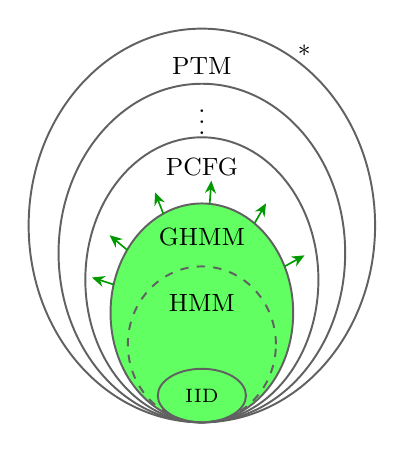
\begin{tikzpicture}[
    ring/.style={draw=black!62,line width=.7pt},
    ghmm/.style={fill=green!62},
    growth/.style={-{Stealth[length=1.6mm,width=1.4mm]},green!60!black,line width=.6pt},
  ]
    % Each class is an oval sitting on a common bottom point at the origin, so
    % containment reads off the nesting: IID inside HMM inside GHMM, and so on.
    \draw[ring] (0,2.50) ellipse[x radius=2.20, y radius=2.50];
    \draw[ring] (0,2.15) ellipse[x radius=1.82, y radius=2.15];
    \draw[ring] (0,1.81) ellipse[x radius=1.48, y radius=1.81];
    \draw[ring,ghmm] (0,1.39) ellipse[x radius=1.16, y radius=1.39];
    \draw[ring,dashed] (0,0.99) ellipse[x radius=0.94, y radius=0.99];
    \draw[ring] (0,0.34) ellipse[x radius=0.56, y radius=0.34];
    % the classes we can currently handle, and the direction of travel
    \foreach \x/\y/\a in {1.05/1.98/29, 0.67/2.53/60, 0.10/2.78/86,
                          -0.49/2.65/111, -0.95/2.19/140, -1.12/1.75/162}{%
      \draw[growth] (\x,\y) -- ++(\a:0.29);}
    \node[font=\small] at (0,4.52) {PTM};
    \node[font=\small] at (0,3.92) {$\vdots$};
    \node[font=\small] at (0,3.24) {PCFG};
    \node[font=\small] at (0,2.36) {GHMM};
    \node[font=\small] at (0,1.52) {HMM};
    \node[font=\scriptsize] at (0,0.34) {IID};
    \node[font=\small] at (1.30,4.72) {$*$};  % see "not exhaustive"
  \end{tikzpicture}
}
\end{minipage}\hfill
\begin{minipage}[c]{0.58\linewidth}
% Expansions of the class acronyms used in hierarchy.tex / hierarchy_green.tex.
% These were lettered down the right-hand side of the original raster; kept as
% text so the slide can size, wrap and search them.
\begin{tabular}{@{}l@{\hspace{1.1em}}l@{}}
  PTM  & Probabilistic Turing Machine           \\[0.3em]
  PCFG & Probabilistic Context-Free Grammar     \\[0.3em]
  GHMM & Generalised Hidden Markov Model        \\[0.3em]
  HMM  & Hidden Markov Model                    \\[0.3em]
  IID  & Independent \& Identically Distributed
\end{tabular}

\end{minipage}
\end{center}
{\small The source diagram marks the region of understood prediction in green
and labels the hierarchy as non-exhaustive.\par}

\subheading{Neural networks}
For what scale of \textbf{neural networks} have we identified the structures
of optimal prediction?
\begin{center}
\renewcommand{\arraystretch}{1.2}
\begin{tabular*}{0.85\linewidth}{@{}l@{\extracolsep{\fill}}r@{}}
\toprule
Architecture & Parameters (approximately)\\
\midrule
Transformer & $10^5$\\
LSTM & $10^5$\\
RNN & $10^4$\\
GRU & $10^5$\\
\bottomrule
\end{tabular*}
\end{center}
Very toy compared to current frontier models ($\sim 10^{12}$)!
\provenance{9--12}
\newpage

\heading{The research frontier and today's scope}
We are working to push the Pareto frontier. We will take a slightly narrower
view and consider:
\begin{center}
\begin{minipage}[t]{0.40\linewidth}
\centering
\resizebox{\linewidth}{!}{% Where the research program has got to: toy->real processes against
% weak->strong models, and the frontier being pushed outward.
% Editable replacement for the pareto.png raster.
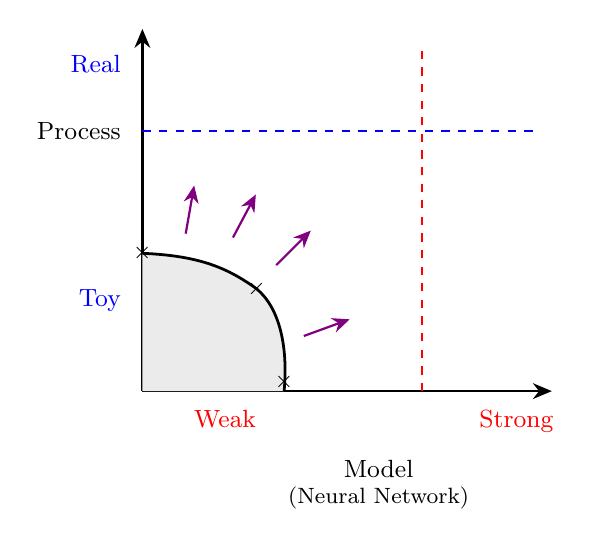
\begin{tikzpicture}[>={Stealth[length=2.4mm,width=2mm]}]
  \draw[->,line width=.9pt] (0,0) -- (0,4.6);
  \draw[->,line width=.9pt] (0,0) -- (5.2,0);
  % what would count as success on each axis
  \draw[blue,dashed,line width=.7pt] (0,3.30) -- (5.0,3.30);
  \draw[red,dashed,line width=.7pt]  (3.55,0) -- (3.55,4.4);
  % the frontier, and what it encloses today
  \fill[black!8] (0,0) -- (0,1.75) .. controls (0.75,1.72) and (1.10,1.55)
                 .. (1.45,1.30) .. controls (1.75,1.05) and (1.85,0.55)
                 .. (1.80,0) -- cycle;
  \draw[line width=1pt] (0,1.75) .. controls (0.75,1.72) and (1.10,1.55)
                 .. (1.45,1.30) .. controls (1.75,1.05) and (1.85,0.55) .. (1.80,0);
  \foreach \p in {(0,1.75), (1.45,1.30), (1.80,0.12)}{\node at \p {\footnotesize$\times$};}
  % direction of travel
  \foreach \s/\a in {(0.55,2.00)/80, (1.15,1.95)/62, (1.70,1.60)/45, (2.05,0.70)/20}{
    \draw[violet,-{Stealth[length=2.2mm,width=1.9mm]},line width=.8pt] \s -- ++(\a:0.62);}
  \node[blue,font=\small,anchor=east] at (-0.15,4.15) {Real};
  \node[blue,font=\small,anchor=east] at (-0.15,1.15) {Toy};
  \node[font=\small,anchor=east]      at (-0.15,3.30) {Process};
  \node[red,font=\small,anchor=north] at (1.05,-0.12) {Weak};
  \node[red,font=\small,anchor=north] at (4.75,-0.12) {Strong};
  \node[font=\small,anchor=north,align=center] at (3.0,-0.75)
       {Model\\[-0.15em]{\footnotesize(Neural Network)}};
\end{tikzpicture}
}
\end{minipage}\hfill
\begin{minipage}[t]{0.56\linewidth}
\centering
\resizebox{\linewidth}{!}{% Today's scope: GHMMs on the process side, transformers on the model side.
% Editable replacement for the scope.png raster; the two halves are drawn in
% one picture so the slide keeps a single \input.
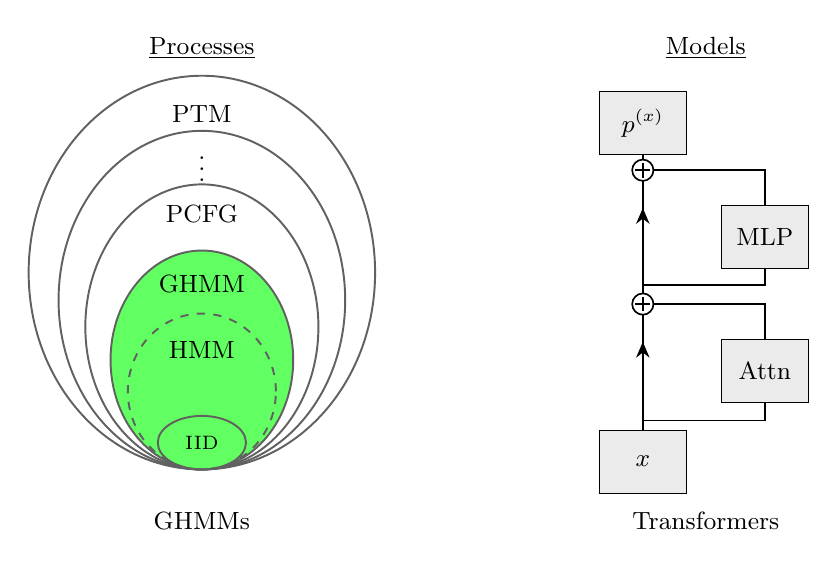
\begin{tikzpicture}[
  ring/.style={draw=black!62,line width=.7pt},
  ghmm/.style={fill=green!62},
  unit/.style={draw,fill=black!8,minimum width=11mm,minimum height=8mm,
               inner sep=1pt,font=\small},
  wire/.style={draw,line width=.6pt},
]
  % ---- processes: the shaded class is the one we tackle ----
  \begin{scope}[shift={(0,0)}]
    \draw[ring] (0,2.50) ellipse[x radius=2.20, y radius=2.50];
    \draw[ring] (0,2.15) ellipse[x radius=1.82, y radius=2.15];
    \draw[ring] (0,1.81) ellipse[x radius=1.48, y radius=1.81];
    \draw[ring,ghmm] (0,1.39) ellipse[x radius=1.16, y radius=1.39];
    \draw[ring,dashed] (0,0.99) ellipse[x radius=0.94, y radius=0.99];
    \draw[ring] (0,0.34) ellipse[x radius=0.56, y radius=0.34];
    \node[font=\small] at (0,4.52) {PTM};
    \node[font=\small] at (0,3.92) {$\vdots$};
    \node[font=\small] at (0,3.24) {PCFG};
    \node[font=\small] at (0,2.36) {GHMM};
    \node[font=\small] at (0,1.52) {HMM};
    \node[font=\scriptsize] at (0,0.34) {IID};
    \node[font=\small] at (0,5.35) {\underline{Processes}};
    \node[font=\small] at (0,-0.65) {GHMMs};
  \end{scope}
  % ---- models: a residual stream, each block writing back into the sum ----
  \begin{scope}[shift={(5.6,0.1)}]
    \node[unit] (x)   at (0,0)    {$x$};
    \node[unit] (px)  at (0,4.30) {$p^{(x)}$};
    \node[unit] (att) at (1.55,1.15) {Attn};
    \node[unit] (mlp) at (1.55,2.85) {MLP};
    \draw[wire] (x.north) -- (px.south);
    \foreach \y in {1.40, 3.10}{\draw[-{Stealth[length=2mm,width=1.7mm]},line width=.6pt]
      (0,\y) -- (0,\y+0.12);}
    \draw[wire] (0,0.52) -- (1.55,0.52) -- (att.south);
    \draw[wire] (att.north) -- (1.55,2.00) -- (0,2.00);
    \draw[wire] (0,2.24) -- (1.55,2.24) -- (mlp.south);
    \draw[wire] (mlp.north) -- (1.55,3.70) -- (0,3.70);
    \foreach \y in {2.00, 3.70}{
      \draw[wire,fill=white] (0,\y) circle[radius=0.135];
      \draw[wire] (-0.093,\y) -- (0.093,\y);
      \draw[wire] (0,{\y-0.093}) -- (0,{\y+0.093});}
    \node[font=\small] at (0.8,5.25) {\underline{Models}};
    \node[font=\small] at (0.8,-0.75) {Transformers};
  \end{scope}
\end{tikzpicture}
}
\end{minipage}
\end{center}

\subheading{Wild Speculation}
As the research program is scale-free one view is that we should develop
the foundations such that future automated AI Safety researchers can
pursue these ideas independently.

\subheading{Plan}
\renewcommand{\arraystretch}{1.4}
\begin{tabularx}{\linewidth}{@{}r@{\hspace{3mm}}X@{\hspace{3mm}}l@{}}
1 & Foundations: Hidden Markov Models & Lecture/exercises\\
2 & Foundations: Prediction & Lecture/exercises\\
3 & Applications: Designing Processes & Tutorial\\
4 & Applications: Belief geometry in transformers & Reading\\
5 & Applications: How do transformers do it? & Tutorial\\
\end{tabularx}

6\hspace{3mm}Q\,\&\,A with Adam Shai and/or Paul Riechers

\subheading{Questions?}
\provenance{13--17}
\end{document}
